% BHU PYQ -- Professional Exam Template
\documentclass[11pt,a4paper]{article}

\usepackage[a4paper,top=2.5cm,bottom=2.5cm,left=2.8cm,right=2.8cm,headheight=14pt]{geometry}
\usepackage{amsmath,amssymb}
\usepackage[T1]{fontenc}
\usepackage[utf8]{inputenc}
\usepackage{lmodern}
\usepackage{microtype}
\usepackage{fancyhdr}
\usepackage{enumitem}
\usepackage{hyperref}
\usepackage{lastpage}
\usepackage{parskip}
\usepackage{tikz}
\usetikzlibrary{arrows.meta,shapes,positioning}

\hypersetup{colorlinks=true,urlcolor=black,linkcolor=black,
  pdftitle={B.Sc. (Hons.) Zoology Sem-VI ZOB-601 -- BHU PYQ}}

\pagestyle{fancy}
\fancyhf{}
\renewcommand{\headrulewidth}{0.4pt}
\renewcommand{\footrulewidth}{0.4pt}
\fancyhead[L]{\small   \textit{Banaras Hindu University}}
\fancyhead[R]{\small   \textit{Zoology Paper: ZOB-601}}
\fancyfoot[C]{\small Page  \thepage\ of \pageref{LastPage}}


\newlist{parts}{enumerate}{2}
\setlist[parts,1]{label=(\alph*),leftmargin=*,itemsep=4pt,topsep=3pt}
\setlist[parts,2]{label=(\roman*),leftmargin=*,itemsep=2pt,topsep=2pt}

\newcommand{\pts}[1]{\hfill   \textit{[#1]}}


\begin{document}


\begin{center}
  {\large\bfseries BANARAS HINDU UNIVERSITY}\\[2pt]
  {
\normalsize B.Sc. (Hons.) Semester VI Examination, 2022-23}\\[6pt]
  \rule{0.8\linewidth}{0.5pt}\\[6pt]
  {\large\bfseries Zoology}\\[4pt]
  {\large\bfseries Paper: ZOB-601 --- Mammalian Physiology}\\[4pt]
  {
\normalsize Time: Three hours \hfill Full Marks: 70}
\end{center}

\rule{\linewidth}{0.4pt}

\smallskip



\noindent   \textit{Note: Answer six questions including Question No. 1 which is compulsory. Draw diagrams wherever necessary. The figures in the right-hand margin indicate marks.}

\bigskip




\noindent   \textbf{Question 1.} Answer the following parts:

\begin{parts}
  \item State whether the following statements are True or False with proper justification:\pts{$8  \times 2 = 16$}
  
\begin{parts}
    \item The initial phase of the repolarization event in the action potential is achieved by opening of the voltage-gated potassium channel.
    \item The visual axis of the human eye crosses through optic disc during image formation.
    \item cGMP-gated Na channel in the cone cell is opened during scotopic vision.
    \item Almost 50\% of the digestion of amylase takes place in buccal cavity.
    \item All the absorption of lipids takes place in small intestine.
    \item Proteins are completely broken into amino acids before absorption.
    \item Transport of sodium ions across luminal membrane involves only antiport transport mechanism.
    \item ATPase action is associated with entire myosin filament.
  \end{parts}
  
  \item Define the following:\pts{$4  \times 1 = 4$}
  
\begin{parts}
    \item Current sink
    \item Tonotopic map
    \item Regurgitation
    \item Anisotropic.
  \end{parts}
\end{parts}

\medskip


\noindent   \textbf{Question 2.} Answer the following:

\begin{parts}
  \item What is membrane potential? Explain, how this is achieved using a suitable diagram.\pts{7}
  
  
\begin{center}
  
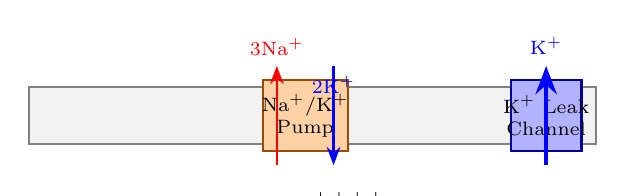
\begin{tikzpicture}[scale=0.9, >=Stealth, every node/.style={font=\small}]
    \draw[fill=gray!10, draw=gray, thick] (-4, 1.0) rectangle (4, 1.8);
    
ode at (0, 1.4) {   \textbf{Lipid Bilayer (Membrane)}};
    
    
ode[above] at (-2, 2.0) {   \textbf{ECF (Extracellular)}};
    
ode[above] at (2, 2.0) {High $ \text{Na}^+$, Low $ \text{K}^+$};
    
ode[below] at (-2, 0.8) {   \textbf{ICF (Intracellular)}};
    
ode[below] at (2, 0.8) {Low $ \text{Na}^+$, High $ \text{K}^+$, $ \text{A}^-$};
    
    \draw[fill=orange!35, draw=orange!60!black, thick] (-2, 0.9) rectangle (-0.8, 1.9) node[pos=0.5, align=center, font=\scriptsize] {$ \text{Na}^+/ \text{K}^+$\\Pump};
    \draw[->, thick, red] (-1.8, 0.7) -- (-1.8, 2.1) node[above, font=\scriptsize] {$3 \text{Na}^+$};
    \draw[<-, thick, blue] (-1.0, 0.7) -- (-1.0, 2.1) node[below, font=\scriptsize] {$2 \text{K}^+$};
    
    \draw[fill=blue!30, draw=blue!60!black, thick] (1.5, 0.9) rectangle (2.5, 1.9) node[pos=0.5, align=center, font=\scriptsize] {$ \text{K}^+$ Leak\\Channel};
    \draw[->, ultra thick, blue] (2.0, 0.7) -- (2.0, 2.1) node[above, font=\scriptsize] {$ \text{K}^+$};
    
    
ode[above, red] at (-3.5, 2.0) {++++};
    
ode[below, blue] at (-3.5, 0.8) {----};
  \end{tikzpicture}
  \end{center}

  \item Explain, how deficiency of vitamin $ \text{B}_{12}$ may lead to Pernicious anaemia.\pts{3}
\end{parts}

\pagebreak

\medskip


\noindent   \textbf{Question 3.} Answer the following:

\begin{parts}
  \item Using a systemic representation, enumerate the events occurring at the neuromuscular junction. Explain, how the above events are associated with Myasthenia Gravis.\pts{6}
  \item Draw a labeled sketch of a Glutamatergic synapse and briefly describe the mode of its functioning.\pts{4}
  
  
\begin{center}
  
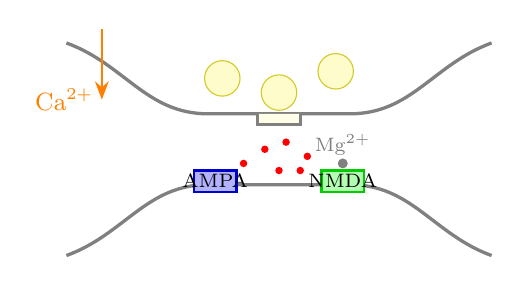
\begin{tikzpicture}[scale=0.9, >=Stealth, every node/.style={font=\small}]
    \draw[very thick, gray] (-3, 3) to[out=-20, in=180] (-1, 2) -- (1, 2) to[out=0, in=200] (3, 3);
    
ode[above] at (-2, 2.7) {Presynaptic};
    
    \draw[very thick, gray] (-3, 0) to[out=20, in=180] (-1, 1) -- (1, 1) to[out=0, in=160] (3, 0);
    
ode[below] at (-2, 0.3) {Postsynaptic};
    
    \draw[fill=yellow!20, draw=yellow!80!black] (-0.8, 2.5) circle (0.25);
    \draw[fill=yellow!20, draw=yellow!80!black] (0.8, 2.6) circle (0.25);
    \draw[fill=yellow!20, draw=yellow!80!black] (0, 2.3) circle (0.25);
    
ode[font=\scriptsize] at (0, 2.3) {Glu};
    
    \draw[very thick, gray, fill=yellow!10] (0.3, 2.0) to[out=-90, in=90] (0.3, 1.85) to[out=-180, in=0] (-0.3, 1.85) to[out=90, in=-90] (-0.3, 2.0);
    
    \foreach \pos in {(-0.2, 1.5), (0.1, 1.6), (0.4, 1.4), (-0.5, 1.3), (0, 1.2), (0.3, 1.2)} {
      \fill[red] \pos circle (1.5pt);
    }
    
ode[red, right] at (0.5, 1.5) {Glutamate};
    
    \draw[fill=blue!30, draw=blue!80!black, thick] (-1.2, 0.9) rectangle (-0.6, 1.2) node[pos=0.5, font=\scriptsize] {AMPA};
    \draw[fill=green!30, draw=green!80!black, thick] (0.6, 0.9) rectangle (1.2, 1.2) node[pos=0.5, font=\scriptsize] {NMDA};
    \fill[gray] (0.9, 1.3) circle (2pt) node[above, font=\scriptsize] {$ \text{Mg}^{2+}$};
    
    \draw[->, thick, orange] (-2.5, 3.2) -- (-2.5, 2.2) node[left] {$ \text{Ca}^{2+}$};
  \end{tikzpicture}
  \end{center}
\end{parts}

\medskip


\noindent   \textbf{Question 4.} Draw a suitably labeled diagram of the human eye retina. Describe the basis of activation of rhodopsin and genesis of photoreceptor potential during dim light vision.\pts{10}


\begin{center}

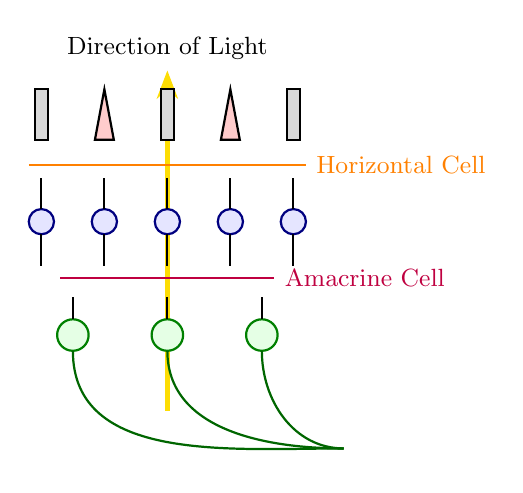
\begin{tikzpicture}[scale=0.8, >=Stealth, every node/.style={font=\small}]
  \draw[->, ultra thick, yellow!80!orange] (0, -2.2) -- (0, 3.2) node[above, black] {Direction of Light};
  
  
\begin{scope}[shift={(0,2.5)}]
    
ode[left] at (-3, 0) {Photoreceptors};
    \foreach \x in {-2, 0, 2} {
      \draw[fill=gray!30, thick] (\x-0.1, -0.4) rectangle (\x+0.1, 0.4);
      
ode[above, font= iny] at (\x, 0.4) {Rod};
    }
    \foreach \x in {-1, 1} {
      \draw[fill=red!20, thick] (\x-0.15, -0.4) -- (\x, 0.4) -- (\x+0.15, -0.4) -- cycle;
      
ode[above, font= iny] at (\x, 0.4) {Cone};
    }
  \end{scope}
  
  
\begin{scope}[shift={(0,0.8)}]
    
ode[left] at (-3, 0) {Bipolar Cells};
    \foreach \x in {-2, -1, 0, 1, 2} {
      \draw[fill=blue!10, draw=blue!50!black, thick] (\x, 0) circle (0.2);
      \draw[thick] (\x, 0.2) -- (\x, 0.7);
      \draw[thick] (\x, -0.2) -- (\x, -0.7);
    }
  \end{scope}
  
  
\begin{scope}[shift={(0,-1.0)}]
    
ode[left] at (-3, 0) {Ganglion Cells};
    \foreach \x in {-1.5, 0, 1.5} {
      \draw[fill=green!10, draw=green!50!black, thick] (\x, 0) circle (0.25);
      \draw[thick] (\x, 0.25) -- (\x, 0.6);
      \draw[thick, green!40!black] (\x, -0.25) to[out=-90, in=180] (2.8, -1.8);
    }
    
ode[right, green!40!black, font=\scriptsize] at (2.8, -1.8) {To Optic Nerve};
  \end{scope}
  
  \draw[thick, orange] (-2.2, 1.7) -- (2.2, 1.7) node[right] {Horizontal Cell};
  \draw[thick, purple] (-1.7, -0.1) -- (1.7, -0.1) node[right] {Amacrine Cell};
\end{tikzpicture}
\end{center}

\pagebreak

\medskip


\noindent   \textbf{Question 5.} Answer the following:

\begin{parts}
  \item A person has met with an accident and has suffered heavy blood loss. Enumerate how the Renin-angiotensin-aldosterone system would respond to regulate blood pressure and fluid balance.\pts{7}
  \item What is impedance match? Briefly explain how this is achieved.\pts{3}
\end{parts}

\medskip


\noindent   \textbf{Question 6.} Answer the following:

\begin{parts}
  \item What is the organ of Corti? Describe its structure and mechanism of function in hearing.\pts{5}
  \item What is Bohr's effect? Explain it by drawing a schematic graph representing the effect of $ \text{CO}_2$ on the oxygen binding affinity of haemoglobin. How is blood pH related to this phenomenon?\pts{5}
  
  
\begin{center}
  
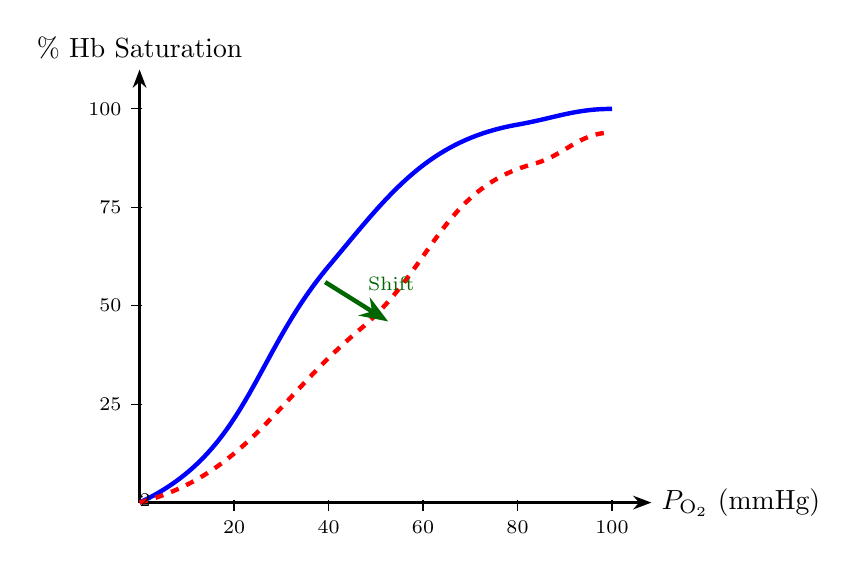
\begin{tikzpicture}[scale=1.0, >=Stealth]
    \draw[->, thick] (0,0) -- (6.5,0) node[right] {$P_{ \text{O}_2} \text{ (mmHg)}$};
    \draw[->, thick] (0,0) -- (0,5.5) node[above] {$\%  \text{ Hb Saturation}$};
    
    \foreach \y/\l in {1.25/25, 2.5/50, 3.75/75, 5.0/100} {
      \draw (1pt,\y) -- (-3pt,\y) node[left, font=\scriptsize] {\l};
    }
    \foreach \x/\l in {1.2/20, 2.4/40, 3.6/60, 4.8/80, 6.0/100} {
      \draw (\x,1pt) -- (\x,-3pt) node[below, font=\scriptsize] {\l};
    }
    
    \draw[ultra thick, blue] (0,0) to[out=25, in=230] (2.4, 3.0) to[out=50, in=190] (4.8, 4.8) to[out=10, in=180] (6.0, 5.0);
    
ode[blue, right] at (4.5, 4.2) {Normal pH (7.4)};
    
    \draw[ultra thick, red, dashed] (0,0) to[out=15, in=220] (2.8, 2.2) to[out=40, in=195] (5.0, 4.3) to[out=15, in=180] (6.0, 4.7);
    
ode[red, right] at (4.5, 2.6) {Low pH / High $ \text{CO}_2$};
    
ode[red, right] at (4.5, 2.15) {(Bohr Effect)};
    
    \draw[->, ultra thick, black!60!green] (2.2, 2.8) -- (3.0, 2.3) node[midway, above right, font=\scriptsize] {Shift};
  \end{tikzpicture}
  \end{center}
\end{parts}

\medskip


\noindent   \textbf{Question 7.} Answer the following:

\begin{parts}
  \item Arrange the respiratory quotients of proteins, carbohydrates and lipids in increasing order and explain the reason behind this difference. Can there be a metabolic situation where the respiratory quotient is more than 1.0? If yes, mention it. If no, explain why.\pts{6}
  \item Describe the cellular content of platelets. How do they contribute towards the formation of a platelet plug?\pts{4}
\end{parts}

\pagebreak

\medskip


\noindent   \textbf{Question 8.} Answer the following:

\begin{parts}
  \item Explain the complete process of digestion, absorption and assimilation of major dietary carbohydrates.\pts{5}
  \item Counter-current mechanism is the main adaptation for the concentration of urine. Explain the mechanism emphasizing on the anatomical features of the loop of Henle and the role of ADH.\pts{5}
\end{parts}

\vfill
\rule{\linewidth}{0.4pt}

\begin{center}\small
\href{https://bhu-exam.vercel.app/}{Click Here}\\[4pt]\href{https://me-aryan.vercel.app/}{Click Here}\\[4pt]\href{https://quashan-me.vercel.app/}{Click Here}
\end{center}

\end{document}
